% Dummy-data draft. Replace the filename and caption after collecting results.
\begin{figure*}[t]
\centering
\includegraphics[width=\textwidth]{figures/evaluation/illustrative_granularity.pdf}
\caption{Illustrative layout for partition-granularity sensitivity.
All values are synthetic placeholders, not experimental results.
Columns correspond to workloads; the top row shows single-request
latency and the bottom row shows sixteen-request batch makespan.
Points represent medians of three synthetic trials; bars show their range.}
\label{fig:eval-granularity}
\end{figure*}

% Measured-data version: use after replacing the CSV with completed trial results.
% \begin{figure*}[t]
% \centering
% 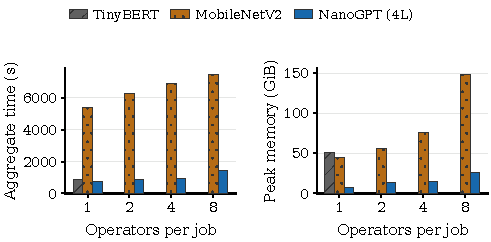
\includegraphics[width=\textwidth]{figures/evaluation/partition_granularity.pdf}
% \caption{Sensitivity of zkInfer to partition granularity under a
% 256~GiB proof-memory budget. Each column corresponds to one workload.
% Setup artifacts are reused, and each partitioning configuration uses
% matching resource profiles. Points show the median across three trials;
% bars show the observed minimum and maximum.}
% \label{fig:eval-granularity}
% \end{figure*}
